\subsection{Predicting Verification Outcomes: Building the Saguaro Cache}
\label{sec:cache_topology}

Given a speculation $\spec^T$ that is in the process of being verified, \Sys must build a cache $\Spec^T$ for the most likely verification outcomes.  
The difficulty is that the space of possible verification outcomes is vast, of size approximately $(K+1)V$ where $V$ is the model vocabulary size.
% While the draft decodes all anticipated speculations at once, in parallel, using a special attention mask (Appendix \ref{app:impl_details}).
Since there are $O(KV)$ potential verification outcomes, it is impractical to preemptively speculate for \textit{all} of them in parallel.
This motivates posing verification prediction as constrained optimization: given a budget of $B$ verification outcomes, how should one select them to maximize the chances of a cache hit?
Note that the budget $B$ typically corresponding to the maximum number of outcomes the draft can finish speculating for before verification completes.
% before the draft model becomes heavily compute bound and thus untenably slow during speculation, 
% how should one select them to maximize the chances of a cache hit? 

\subsubsection{Algorithm}
\label{sec:cache_topology_alg}

\begin{wrapfigure}{l}{0.4\linewidth}
  \vspace{-20pt} % reduce space below
  \centering
    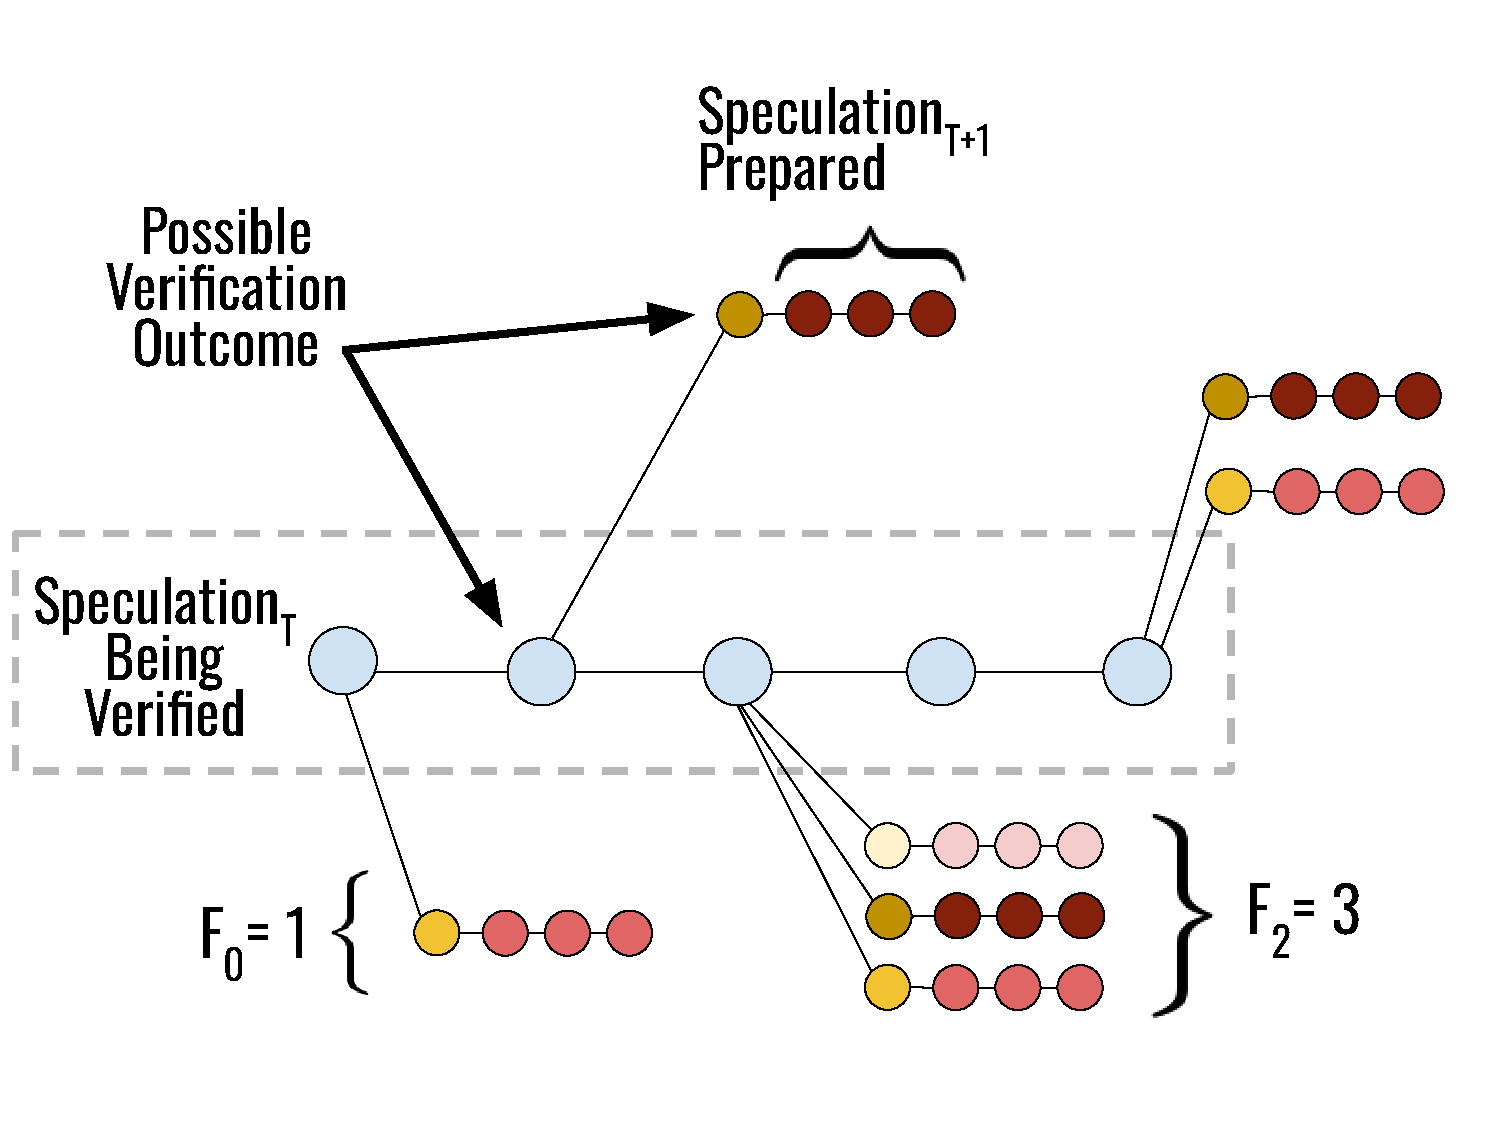
\includegraphics[width=\linewidth,height=0.7\linewidth,keepaspectratio]{figures/fan_out_simple_1.pdf}
  \caption{Schematic of speculation cache strategy. We allocate \textit{fan-out} $F_k$ (bonus token guesses) over sequence length $K+1$ according to Theorem \ref{thm:cache_topology}.}
  \vspace{-30pt} % reduce space below
\end{wrapfigure}

\begin{definition}
We define the \textbf{fan-out} $F_k^p := \big| \{ v^T \coloneqq (k',t^*) \in \Spec^T \;\mid\; k'=k \} \big|$ at position $k$ to be the number of verification outcomes with $k$ accepted tokens that are included in the speculation cache, given the previous iteration was speculated by the primary speculator. $F_k^b$ is defined analogously for the \textit{backup} speculator. 
\end{definition}

\paragraph{Saguaro Verification Outcome Prediction Algorithm}

Given a fan-out strategy $\{F_k^p, F_k^b\}$ (ours based on Theorem \ref{thm:cache_topology}), \Sys takes the top-$F_k$ tokens at each lookahead position $k$ in the draft logits, and adds those to the speculation cache.
These are the top-$F_k$ logits \textit{excluding} the sampled token sent for verification at that position, which is \textit{guaranteed} not to be the bonus token.


\subsubsection{Theoretical Results}
\label{sec:cache_topology_theory}
We show how to optimize the choice of fan-out values $F_k^p$ and $F_k^b$ to maximize the speedup under a constraint on the size of the speculation cache.


The probability of a verification outcome $(k, \cdot)$ in a given iteration depends on whether the previous speculation was generated by the primary or backup speculator. 
Thus, if the default fan-out strategy when building the cache is to fan out uniformly at each sequence position, the cache hit rate on a given iteration depends on whether the previous iteration was speculated by the primary or backup speculator. 
These are the definitions of $p_{\mathrm{hit,p}}(F)$ and $p_{\mathrm{hit,b}}(F)$, respectively. 
We see in Figure~\ref{fig:phits} that these functions (in fact their complement, the rejection rate) empirically follow a power-law. 

\begin{definition}\hspace{-0.05in}\footnote{
        This definition is closely related to the notion of $b$ power-law acceptance rate in \cite{sequoia}.
    }
    \;We say that a speculator has a \textbf{$\mathbf{r}$ power-law cache hit rate} if the chance of a cache miss with fan-out $F$ is equal to a power-law of $F$ with exponent $r$, for a sequence drafted by this speculator.
    More specifically, this means $1-p_{\mathrm{hit,*}}(F) = 1/F^r \;\; \forall F \in \mathbb{N}$, for some $r > 0$.
\end{definition}

We now use this definition to reason about how to optimally select the fan-out values $F_k^p$ and $F_k^b$ under a computational constraint on the size of the cache. 
We consider the general case, when this assumption doesn't hold, in Appendix~\ref{app:theory}.

\begin{theorem}
\label{thm:cache_topology}
\textbf{(\Sys Cache Shape: Geometric Fan-Out)} Consider a draft model with acceptance rate $a_p$ and a $r$ power-law cache hit rate.
Then  the optimal choice of $F_k^p$ values for $k\in [0,K]$ under the constraint $\sum_{k=0}^K F_k^p \leq B$, follows a capped geometric series:
\begin{eqnarray*}
F_k &=& F_0 \cdot a_p^{k/(1 + r)}  \;\; \forall k < K, \; \text{and} \\
F_K &=& F_0 \cdot a_p^{K/(1 + r)} \cdot (1-a_p)^{-1/(1 + r)},
\end{eqnarray*}
where $F_0$ can be chosen such that $\sum_{k=0}^K F_k^p = B$ (closed form-equation in Appendix~\ref{app:theory}).
An equivalent result holds for $F_k^b$. 
\end{theorem}

This result cleanly reflects the intuition that the lengths of verified strings follow a capped geometric distribution supported on the speculation lookahead. In other words, if it is unlikely that $j \in [0, K]$ tokens will be accepted by the verifier, we should not waste compute guessing and speculating on the bonus token at that position, and should lower $F_j$. 

\subsubsection{Empirical Evaluation}

We compare the end-to-end performance of using a naive (uniform) fan-out strategy over sequence length against the geometric fan-out strategy advanced by Theorem \ref{thm:cache_topology}.
In Figure \ref{fig:geom} we find it improves cache hit rate (right) and end-to-end decoding speed, especially at higher temperatures, where both SD and the uniform fan out begin to flounder.

\begin{figure}[ht]
    \centering
    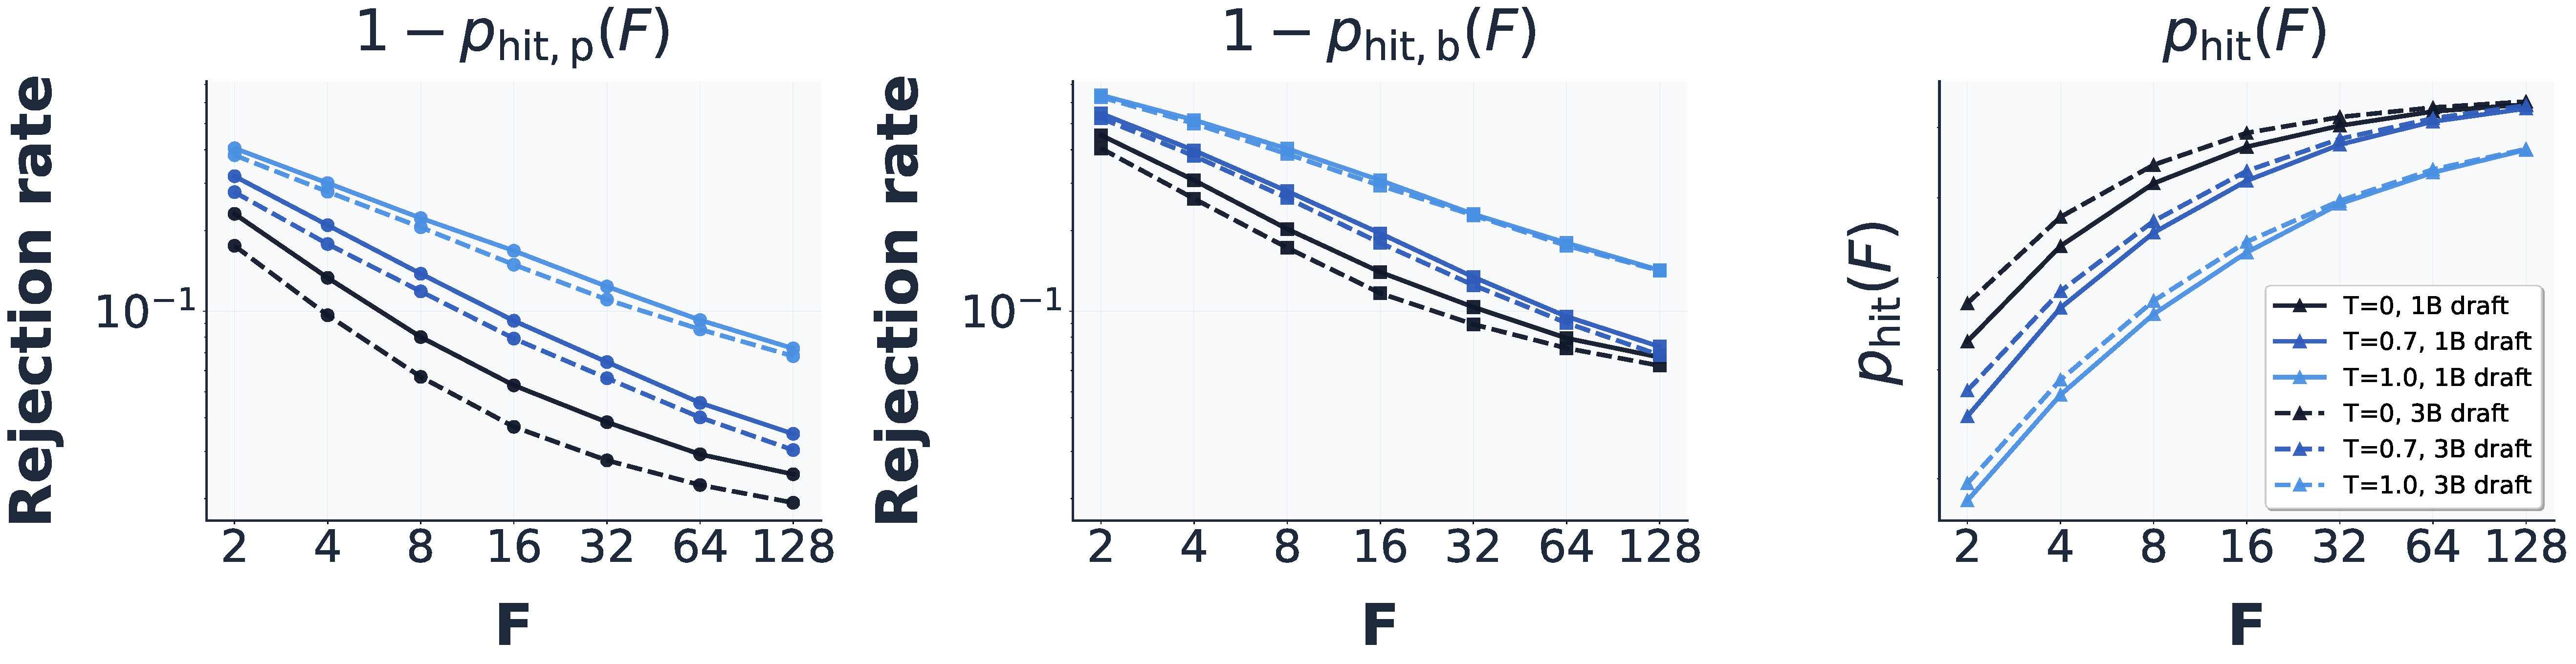
\includegraphics[width=\linewidth]{figures/dts_analysis_final.pdf}
    \caption{
        Scaling of cache hit rates with fan out.
        (Left, middle) The rejection rates (1 - $p_{hit,*}(F)$) conditioned on the prior speculation coming from the primary vs backup speculator, respectively.
        Rejection rates (cache misses) fall as a power law in the draft-fan out, demonstrating that cache hit rates increase with cache size.
        (Right) The overall cache hit rate $p_\text{hit}(F)$.
    }
    \label{fig:phits}
\end{figure}

\begin{figure}[ht]
    \centering
    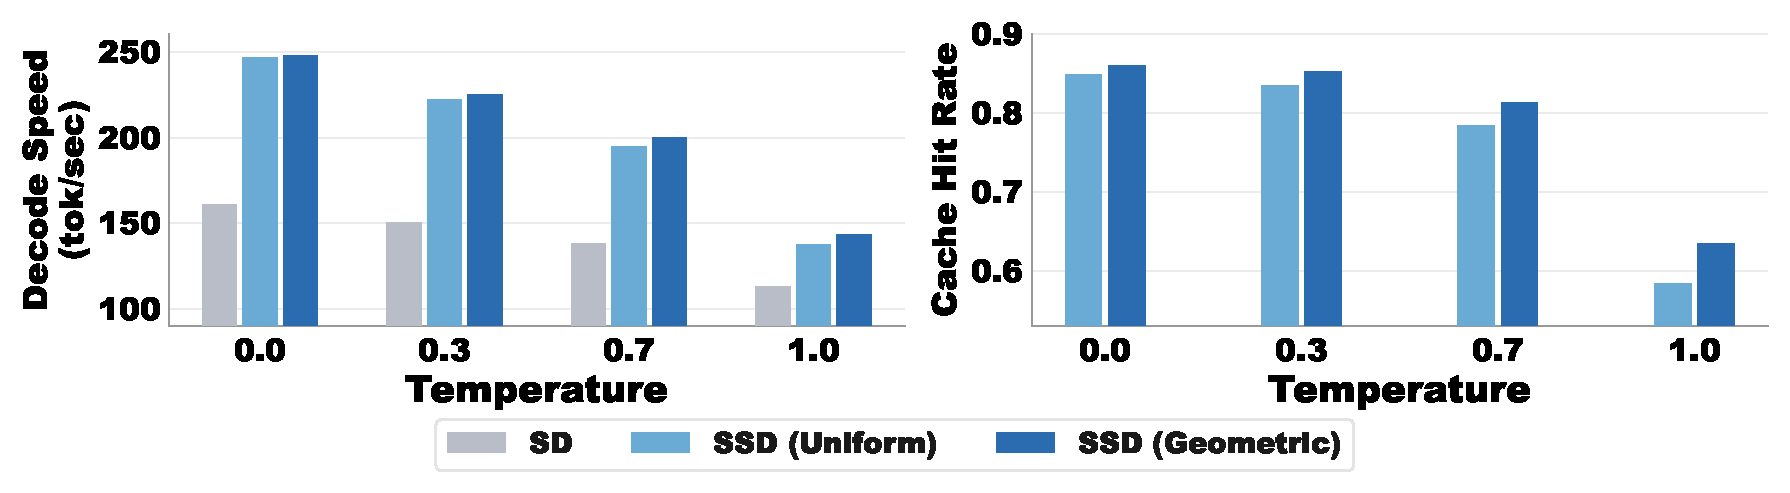
\includegraphics[width=0.9\linewidth]{figures/temp_fan_out_llama.pdf}
    \caption{Advantage of geometric fan out strategy increases at higher temperatures, improving both speculation cache hit rate (right) and thus end-to-end speed (left). Results averaged over four datasets. At all temperatures, SSD with either fan out strategy outperforms ordinary speculative decoding. }
    \label{fig:geom}
\end{figure}
